\documentclass{standalone}
\usepackage{tikz}

\usetikzlibrary{calc}


\begin{document}

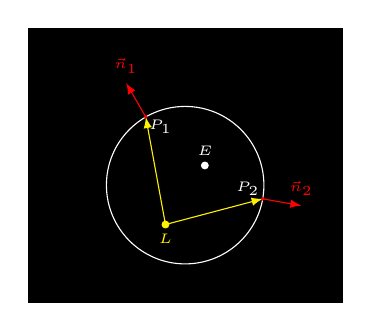
\begin{tikzpicture}
  \path[fill=black] (-2,-1.5) rectangle (2,2);
  \draw[white] (0,0) circle [radius=1cm];

  \coordinate (P1) at (120:1);
  \coordinate (P2) at (-10:1);
  \coordinate (L) at (-0.25,-0.5);
  \coordinate (E) at (0.25,0.25);

  \path[fill=yellow] (L) circle [radius=0.05cm] node[below,font=\tiny,yellow] {$L$};
  \draw[yellow,-latex] (L) -- (P1);
  \draw[yellow,-latex] (L) -- (P2);

  \path[fill=red] (P1) circle [radius=0.025cm] node[anchor=north west,inner sep=1pt,font=\tiny,white] {$P_1$};
  \path[fill=red] (P2) circle [radius=0.025cm] node[anchor=south east,inner sep=1pt,font=\tiny,white] {$P_2$};

  \draw[-latex,red] (P1) -- ($ (0,0) ! 1.5 ! (P1) $) node[above,font=\tiny] {$\vec n_1$};
  \draw[-latex,red] (P2) -- ($ (0,0) ! 1.5 ! (P2) $) node[above,font=\tiny] {$\vec n_2$};

  \path[fill=white] (E) circle [radius=0.05cm] node[above,font=\tiny,white] {$E$};
\end{tikzpicture}

\end{document}